\providecommand{\main}{..}
\documentclass[\main/master.tex]{subfiles}
\begin{document}
\chapter{Theoretical background}\label{chapter:Theoretical background}

\section{Torsional pendulum}
\subsection{Torsional pendulum}
\begin{figure}[htbp]
	\centering
	\fbox{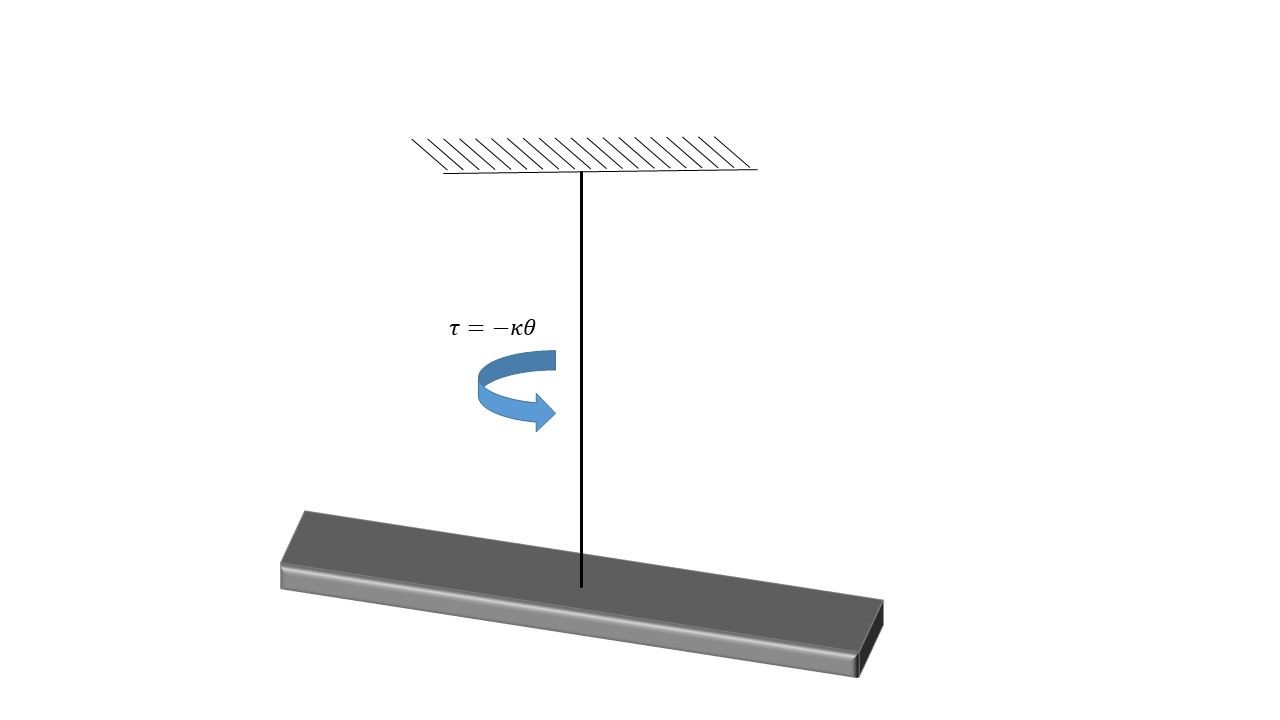
\includegraphics[scale=0.4]{\main/images/2 - theoretical background/torsion_pendulum_powerpoint.jpg}}
	\caption[Torsional pendulum]{A torsional pendulum}
	\label{fig:torsion_pendulum}
\end{figure}
\par\noindent
A torsional pendulum, shown in fig.~\ref{fig:torsion_pendulum}, is an oscillator made of a mass hung by a string from a fixed point allowing it to swing freely. When the mass is displaced from the equilibrium angle, the pendulum has a linear restoring torque, caused by the twisted string. 
\par\noindent
The restoring torque $\tau$, which is proportional to the string torsion coefficient $\kappa$, rotates the mass back to the equilibrium position:
\begin{equation}
\tau = -\kappa\cdot\theta     \label{eqn:undamped_motion_equation}
\end{equation}

\par\noindent
Assuming homogeneity of a circular string, the string torsion coefficient $\kappa$ can be estimated:
\begin{equation}
\kappa = \frac{GJ}{h} = \frac{G}{h} \frac{\pi d^4}{32}    \label{eqn:torsion_coefficient_homogeneity}
\end{equation}
\par\noindent
Where $G$ is the material shear modulus, $J$ is the circular second moment of area ($Jzz$), $h$ is the string length and $d$ is the string diameter.
 


\subsection{Simple harmonic oscillator}
The harmonic oscillator is a second order system that, when displaced, experiences a linear restoring force proportional to the displacement from equilibrium. The torsional pendulum is an angular harmonic oscillator. However, it is equivalent to the linear case, where instead of velocity and force, one has angular velocity and torque.
\par\noindent
If the restoring torque is the only torque in action, then the oscillator is not driven or damped oscillator, resulting in a simple harmonic motion:
\begin{equation}
\tau = -\kappa\cdot\theta  = I\cdot\ddot{\theta}   \label{eqn:undamped_motion_equation}
\end{equation}
\par\noindent
Where $I$ is the moment of inertia of the torsional pendulum. 
\par\noindent
Solving eq.~\ref{eqn:undamped_motion_equation}, the torque causes sinusoidal oscillations (simple harmonic motion) around the equilibrium angle:  
\begin{equation}
\theta(t) = \theta_{max}cos(\omega_0 t )    \label{eqn:undamped_motion_equation_solved}
\end{equation}
\begin{equation}
\omega_0  = \frac{2\pi}{T} = \sqrt{\frac{\kappa}{I}}   \label{eqn:undamped_omega}
\end{equation}
\par\noindent
Where $\omega_0$ is the natural resonant frequency, and $T$ is the time period of oscillation, $\omega_0$ and $T$ are determined by the physical constants of the pendulum $\kappa$, $I$. Accordingly, the string torsion coefficient $\kappa$ could also be found empirically by finding the oscillations period $T$.


\subsection{Damped oscillator}
If the system also has damping torque (a friction), the system is a damped oscillator: 

\begin{equation}
\tau_{drag} = -b\cdot\dot{\theta}   \label{eqn:friction_torque}
\end{equation}
The damping torque, is proportional to the angular velocity, where $b$ is the oscillator damping coefficient. 
\par\noindent
Thus, eq.~\ref{eqn:undamped_motion_equation} becomes:
\begin{equation}
\tau = -\kappa\cdot\theta - b\dot{\theta}  = I\cdot\ddot{\theta}   \label{eqn:damped_motion_equation}
\end{equation}
Eq.~\ref{eqn:damped_motion_equation} could be rewritten as:
\begin{equation}
\ddot{\theta} + 2\xi\omega_0\dot{\theta} + \omega_0^2\theta = 0   \label{eqn:damped_motion_equation_2}
\end{equation}
Where, $\xi$ is the oscillator damping ratio, which determines the oscillator damping type and damping time. The damping ratio is given by:
\begin{equation}
\xi = \frac{b}{2\sqrt{I\kappa}} 
\label{eqn:system damping ratio}
\end{equation}
The damping time $\tau$ is given by:
\begin{equation}
\tau = \frac{1}{\xi\omega_0} = \frac{1}{\frac{b}{2\sqrt{I\kappa}}\sqrt{\frac{\kappa}{I}} }= \frac{2I}{b}  \label{eqn:damping_time}
\end{equation}

\par\noindent
Solving eq.~\ref{eqn:damped_motion_equation_2}, the oscillator could be either undamped, overdamped, critically damped or underdamped. 
\par\noindent
The motion equations when boundaries are $\theta(0) = \theta_{max}$ and $\dot{\theta}(0) = 0$:

\par\noindent
When $\xi = 0$ the oscillator is undamped; there is no friction and damping, leading to harmonic oscillations without decay.
\begin{equation}
\theta(t) = \theta_{max}cos(\omega_0 t )    \label{eqn:undamped_motion_equation}
\end{equation}
When $\xi < 1$ the oscillator is underdamped; amplitude of the oscillations decreases in time due to the friction while oscillating with a lower frequency due to the damping. 
\begin{equation}
\theta(t) = \theta_{max} e^{-\frac{t}{\tau}}cos(\sqrt{1-\xi^2}\omega_0 t ) =  \theta_{max} e^{-\frac{t}{\tau}}cos(\omega t )    \label{eqn:underdamped_motion_equation}
\end{equation}
When the damping coefficient is small enough, the frequency change is negligible, and can be approximated by:
\begin{equation}
\omega = \omega_0\sqrt{1-\xi^2}\approx\omega_0    \label{eqn:underdamped_frequency}
\end{equation}
\par\noindent
When $\xi = 1$ the oscillator is critically damped; due to high friction, the system cannot oscillate and it decays exponentially to the equilibrium position. For a fixed $I, \kappa$, choosing $b$ to be at the critical damping value would give the fastest return to the equilibrium position. 
\begin{equation}
% A+B t (e^{-\frac{t}{\tau}}) 
\theta(t) = \theta_{max}(1+\frac{t}{\tau}) e^{-\frac{t}{\tau}}     \label{eqn:underdamped_motion_equation}
\end{equation}
\par\noindent
When $\xi > 1$ the oscillator is overdamped; when there is high friction, the system cannot oscillate and it decays exponentially to the equilibrium position. 
\begin{equation}
\theta(t) = \frac{\theta_{max}}{2} [ (1-\xi')e^{-\frac{t}{\tau}(1+\frac{1}{\xi'})} +(1-\xi')e^{-\frac{t}{\tau}(1-\frac{1}{\xi'})} ]
\label{eqn:overdamped_motion_equation}
\end{equation}
where 
\begin{equation}
\xi'  = \frac{\xi}{\sqrt{\xi^2 - 1}}  \label{eqn:overdamped_motion_equation}
\end{equation}
\iffalse
\begin{equation}
\theta(t) = Ae^{-\frac{t}{\tau}(1+\sqrt{1-\frac{1}{\xi^2}})} + Be^{-\frac{t}{\tau}(1-\sqrt{1-\frac{1}{\xi^2}})}    \label{eqn:overdamped_motion_equation}
\end{equation}
\fi 
\par\noindent
Fig.~\ref{fig:damped_oscillators} shows the amplitude of the oscillations of the different damping types.
\begin{figure}[htbp]
	\centering
	\fbox{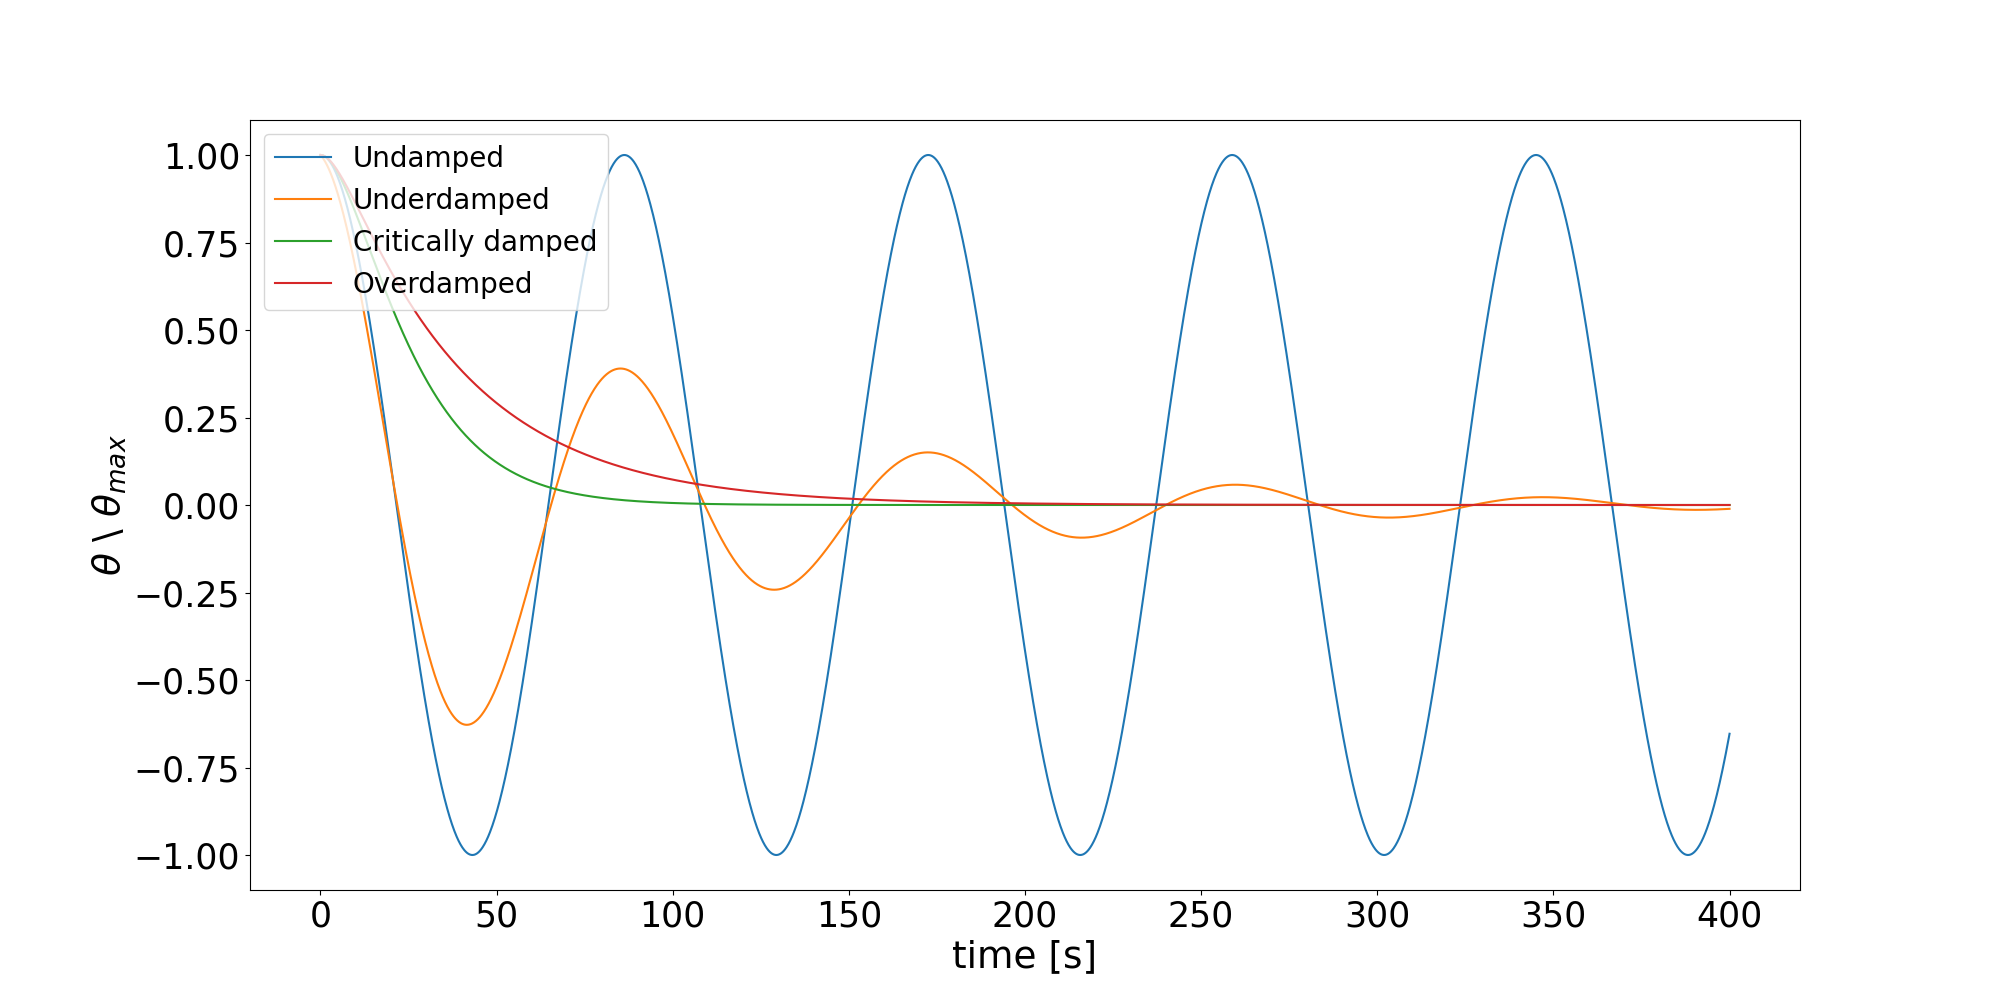
\includegraphics[scale=0.7]{\main/images/2 - theoretical background/damp.png}}
	\caption[Damped oscillators comparison]{Damped oscillators comparison}
	\label{fig:damped_oscillators}
\end{figure}
\FloatBarrier
\iffalse
https://ocw.mit.edu/courses/mathematics/18-03sc-differential-equations-fall-2011/unit-ii-second-order-constant-coefficient-linear-equations/damped-harmonic-oscillators/MIT18_03SCF11_s13_2text.pdf

https://www.sciencedirect.com/topics/engineering/underdamped-system#:~:text=When%20the%20damping%20ratio%20is%20between%200%20and%201%20(i.e.,is%20an%20exponential%20decay%20line.
\fi


\subsubsection{Driven oscillator}
If the damped oscillator system is further affected by an external time-dependent torque $\tau(t)$, the system is known as a driven oscillator, and its motion equation is:
\begin{equation}
\tau(t) -\kappa\cdot\theta - b\dot{\theta}  = I\cdot\ddot{\theta}   \label{eqn:driven_motion_equation}
\end{equation} 
Eq.~\ref{eqn:driven_motion_equation} could be rewritten as:
\begin{equation}
\ddot{\theta} + 2\xi\omega_0\dot{\theta} + \omega_0^2\theta = \frac{\tau(t)}{I}   \label{eqn:damped_motion_equation}
\end{equation}






\section{Gravity measurement}
\subsection{Gravitational field}
Newton's law of universal gravitation states that every mass $M$ attracts every other mass $m$ in the universe by force $F$ given by:
\begin{equation}
\overrightarrow{F}(r) = \frac{GMm}{r^2}\hat{r}    \label{eqn:gravitation_force}
\end{equation}
Where $G$ is the gravitational constant, and $r$ is the distance between the centers of the masses. The force $F$ acts along the intersecting line, inverse to the square of the distance $r$, causing the force to be very weak. For example, the force between two cubes 1 kg each, 1 meter apart would be $\overrightarrow{F} = 6.67\cdot10^{-11} [N]$.
\par\noindent
The gravitational field $g$ of mass $M$ is defined as the force per unit mass, which is a vector field consisting, at every point, a vector pointing directly towards the particle. The magnitude of the field at every point is calculated by applying the universal law. 
\begin{equation}
\overrightarrow{g}(r) = \frac{\overrightarrow{F}(r)}{m} = \frac{GM}{r^2}\hat{r}    \label{eqn:gravitation_field}
\end{equation}
\subsubsection{Field measurement}
\par\noindent
The field caused by a test mass $M$ at a specific point is calculated by measuring the gravitational force acting on known mass $m$. In general, test mass $M$ is much larger than mass $m$, ensuring a negligible influence on the behavior of $M$.  

\subsection{Cavendish experiment}
\subsubsection{Apparatus}
\begin{figure}[htbp]
	\centering
	\fbox{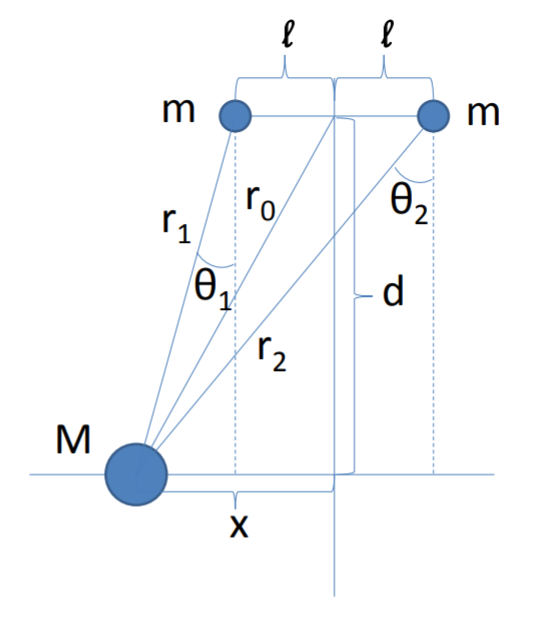
\includegraphics[scale=1]{\main/images/2 - theoretical background/Cavendish apparatus.PNG}}
	\caption[Cavendish apparatus]{Cavendish apparatus \cite{howell2019}}
	\label{fig:Cavendish apparatus}
\end{figure}
%\FloatBarrier
\par\noindent
The Cavendish experiment, first performed in the 17th century, was the first experiment to measure the gravitational force between masses. 
\par\noindent
The apparatus, shown in fig.~\ref{fig:Cavendish apparatus}, is constructed by a torsional pendulum and a nearby test mass $M$, creating a net torque on the pendulum. 
\par\noindent
The pendulum can be assumed to be consisted of two masses $m$ connected by a rigid, massless thin rod, with length of $2l$, and a pivot point at distance $l$ from each mass.
\par\noindent
The pendulum moment of inertia oscillating around the pivot is:
\begin{equation}
I = 2ml^2     \label{eqn:moment_inertia}
\end{equation} 
\subsubsection{gravitational torque}
The mass $M$, located at distance $r_0$ from the pivot point attracts the two masses and creates torques. The net gravitational torque $\tau_g$ for a balanced torsional pendulum is the sum of two inverse, nearly counterbalancing, gravitational torques, one from each mass $m$:
\begin{equation}
\tau_g = l \cdot F(r_1) \cdot cos\theta_1 - l \cdot F(r_2) \cdot cos\theta_2 = l d GmM(\frac{1}{r_1^3} - \frac{1}{r_2^3})     \label{eqn:net_gravitation_torque}
\end{equation}
Defining the function $h(l)$:
\begin{equation}
h(l) = \frac{1}{(d^2 +(x-l)^2)^{3/2}} \label{eqn:gravitation_torque}
\end{equation}
Where $h(l) = \frac{1}{r_1^3},\quad	h(-l) = \frac{1}{r_2^3},\quad	h(0) = \frac{1}{r_0^3}$, and $h'(0) = \frac{3x}{r_0^5}$. Since $l<<d,x,r_0$ one can approximate:
\begin{equation}
h(l)-h(-l)\approx h'(0)\cdot 2l = \frac{6lx}{r_0^5}\label{eqn:approximation}
\end{equation}
According to eq.~\ref{eqn:net_gravitation_torque}, the net torque is proportional to the difference of the functions $h(l)-h(-l)$:
\begin{equation}
\tau_g = l d GmM[h(l)-h(-l)]\approx \frac{6l^2GmMxd} {r_0^5} = \frac{6l^2GmM sin\theta cos\theta}{r_0^3}      
\label{eqn:net_gravitation_torque_approx}
\end{equation}
Where $\theta$ is the tilt angle of the torsional pendulum and approximately $\theta_1 \approx \theta_2 = \theta$.
\subsubsection{Simple harmonic oscillator}
Assuming no friction or other damping force (simple harmonic motion) when a test mass $M$ is introduced, there are two sources of torque in the system; the net torque caused by the gravitational force $\tau_g$ (eq.~\ref{eqn:net_gravitation_torque_approx}), and a restoring torque at the opposite direction caused by the wire torsion (eq.~\ref{eqn:undamped_motion_equation}):
\begin{equation}
\tau = \tau_g - \kappa\theta     \label{eqn:gravitation_torque}
\end{equation}
\par\noindent
As seen previously in eq.~\ref{eqn:undamped_omega}, for a torsional pendulum:
\begin{equation}
\kappa = I\omega_0^2 = (2ml^2)(\frac{2\pi}{T})^2     \label{eqn:moment_inertia}
\end{equation} 
\par\noindent
At equilibrium, the two sources of torque cancel each other out:
\begin{equation}
\kappa\theta = \tau_g    \label{eqn:gravitation_torque}
\end{equation}
Accordingly, $\overline{\theta}$ the average equilibrium tilt angle of torsion is:
\begin{equation}
\overline{\theta} = \frac{\tau_g}{\kappa}  \approx \frac{6l^2GmMcos\theta sin\theta}{2ml^2 (\frac{2\pi}{T})^2 r_0^3}   \label{eqn:theta average}
\end{equation} 
\begin{equation}
\overline{\theta}  \approx \frac{3GT^2cos\theta sin\theta}{4\pi^2 } \cdot \frac{M}{r_0^3}   \label{eqn:theta average_2}
\end{equation}
\par\noindent
The pendulum equilibrium angle is proportional to the square of the period's length $T$, the pendulum length $l$ and the masses $m$ are dropped out, indicating that short and light weight sensors work well as larger ones, as long as their periods are the same.
\par\noindent
According to eq.~\ref{eqn:theta average_2}, by accurate angle measurement, the gravitational field could be estimated.
 

\subsection{Gravity sensing}
The field at a specific point is the superposition of multiple fields, caused by any mass in space $M$ acting on mass $m$ located at that point. Measuring the gravitational field caused by a specific test mass $M$ accurately with known mass $m$, the test mass $M$ weight or its distance could be estimated. In order to filter out the other gravitational fields caused by masses around, one measures the difference from a baseline state.
\par\noindent
Usually the measurement is based on measuring oscillation frequency. The test mass oscillates in different frequencies, where not moving would be zero frequency. The masses around that do not move, are filtered out.
\par\noindent
The sensor's tilt angle caused by the gravitational field is measured at each frequency, measuring the energy spectral density $[\frac{rad}{\sqrt{Hz}}]$ of the sensor.
In the measurement system different noises have different frequencies. By integrating over long periods, measurement noises are reduced. The signal to noise ratio (SNR) is the limiting factor for the sensitivity of a measuring system. In higher frequencies the integration is faster, causing less noises and higher SNR.
The dependency of the SNR on frequency causes difficulties when measuring gravitational fields at low frequencies.
\par\noindent
This limitation is a significant challenge while designing gravimetric sensors for low frequencies.

\subsubsection{The shot noise limit}
A optical measurement system can not measure a signal smaller than its shot noise, which is a fundamental quantum physical phenomenon. The power of an optical signal fluctuates due to fluctuations in the number of photons $N$ in the signal. The SNR of a shot noise limited system is:
\begin{equation}
SNR = \frac{N}{\sqrt{N}} = \sqrt{N}    \label{eqn:shot_noise}
\end{equation}
However, while other system noises are higher than the shot noise limit, reducing noises and averaging the time integration can provide higher accuracy and better measurement results. 

\section{Radiation-pressure}
Radiation-pressure is the pressure of a light beam on the surface due to momentum exchange with the electromagnetic field. The momentum exchange may occur with light at any wavelength which is absorbed, reflected, or emitted by the surface. The pressure causes a force on the surface, although this force is usually insignificant.
  
\par\noindent
The radiation-pressure force depends on the surface angle relative to the electromagnetic field propagating direction, as well as the surface reflectance and absorbance, and the power of light hitting the surface $\Theta_i$ (radiant flux, measured in watts). 
\par\noindent
Assuming that the beam is focused tightly enough that variation over the surface is negligible, the incident radiation pressure is:
\begin{equation}
P_{incident} = \frac{\frac{\Theta_i}{A}cos^2(\alpha)}{c} = \frac{\eta\cdot \Theta_{source}\cdot cos^2(\alpha)}{{A\cdot c}} \label{eqn:radiation_pressure}
\end{equation}
Where $\alpha$ is the field angle, compared to the surface area $A$, $c$ is the speed of light and $\eta$ is the coupling efficiency due to light losses. The light losses are caused by the light beam passing through light transmitters (such as light guide or fiber), and size difference between the light beam size and the target size. 
\par\noindent
When the light field direction is perpendicular to the surface or the angle of the incident is negligible the radiation pressure is:
\begin{equation}
P_{incident} = \frac{\eta\Theta_{source}}{{Ac}} \label{eqn:radiation_pressure_perpendicular}
\end{equation}
\par\noindent
For a reflective material with reflectivity $R$, the radiation force is:
\begin{equation}
F = P_{total}\cdot A = (P_{incident}+P_{reflected})\cdot A = P_{incident}(1+R)A \label{eqn:radiation_force}
\end{equation}
For a material with high reflectivity, $R\approx 1$:
\begin{equation}
F \approx 2P_{incident}A = \frac{2\eta\Theta_{source}}{{c}}\cdot \frac{A}{A} \label{eqn:radiation_force_reflective}
\end{equation}
Thus:
\begin{equation}
F = \frac{2\eta\Theta_{source}}{{c}} \label{eqn:radiation_force_power}
\end{equation}

\section{Vacuum affects}

\subsection{Brownian motion}
Brownian motion is the pattern of random particles' fluctuations at fluid or gas phases, a random walk with no preferential direction of flow. This pattern happens at thermal equilibrium in a given temperature (on average there is no linear and angular momentum). 
\par\noindent
According to the ideal gas law: 
\begin{equation}
N k_B T = PV  \label{eqn:ideal-gasses}
\end{equation}
Where $N$ is the number of particles inside the medium, $k_B$ is the Boltzmann constant, $T$ is the temperature, $P$ is the gas pressure and $V$ is the medium volume. Thus, when medium volume $V$ is constant, the gas pressure is proportional to the number of particles.
\par\noindent
The Maxwell-Boltzmann distribution of molecular speed is:
\begin{equation}
f(v) = 4\pi(\frac{m}{2 \pi k_B T})^{3/2}\cdot v^2\cdot exp(\frac{-mv^2}{2kk_BT})     \label{eqn:Maxwell_Boltzmann}
\end{equation} 
\par\noindent 
Thus, the average kinetic energy for a gas particle is: 
\begin{equation}
<E_k>=<\frac{mv^2}{2}> = \int_{0}^{\infty}\frac{mv^2}{2}f(v)dv =  \frac{3k_BT}{2}    \label{eqn:average_kinetic}
\end{equation}
\par\noindent
Thus, the total Brownian motion energy is:
\begin{equation}
E_k = N<E_k> =\frac{3}{2}N k_B T = \frac{3}{2}PV    \label{eqn:total_kinetic}
\end{equation}
\par\noindent
Eq.~\ref{eqn:total_kinetic} shows that the Brownian motion energy is proportional to the number of gas particles inside the medium. Reducing the gas pressure (having vacuum), which reduces the number of gas particles results with a reduction in the total Brownian motion energy. Since there is thermal energy coupling from the environment on the sides of the medium, reducing the number of particles reduces the energy coupling.
\subsubsection{Brownian uncertainty}
The Brownian motion kinetic energy is proportional to the temperature. The noise of quantum uncertainty due to Brownian motion at a given temperature is: 
\begin{equation}
\frac{1}{2}\kappa (\delta\theta)^2= \frac{1}{2}k_BT  \label{eqn:radiation force}
\end{equation}
\begin{equation}
\delta\theta = \sqrt{\frac{k_BT}{\kappa}}\propto{T}  \label{eqn:radiation force}
\end{equation}

\subsection{Drag}
The friction caused by gas resistance, which is dependent on the relative velocity between the gas and the object. 
At the turbulent flow regime, the gas resistance is proportional to the square of the relative velocity: 

\begin{equation}
F_{drag} = -b\cdot v  \label{eqn:energy-mass-equivalence-relation}
\end{equation}
\par\noindent
When Knudsen ratio is $0.01<k_n<0.5$, at a medium vacuum regime, the flow is called Knudsen flow. The molecules do not interact and move in straight lines between points. If chamber vacuum level is medium or higher, classical viscous friction of objects with gas particles inside the chamber could be negligible.

\subsubsection{Flow characteristics}
Gas pressure at a medium is inverse to the mean free pass of each particle. A gas particle collides many times along it's way. It's mean free path is the average distance the particle could pass between two collisions with other particles. 


\begin{equation}
I = \frac{k_B\cdot T}{\sqrt{2}\cdot\pi\cdot p\cdot d_m^2}     \label{eqn:mean-free-pass}
\end{equation}
The Knudsen ratio, derived from the above term, is used to characterize types of gas flow compare to the pipe diameter.
\begin{equation}
K_n = \frac{I}{d}     \label{eqn:mean-free-pass}
\end{equation}

\subsection{Acoustic wave}
Acoustic waves are energy propagating through material, by adiabatic compression and decompression. The equation of one dimension acoustic wave, where the amplitude is acoustic pressure is:
\begin{equation}
P-P_0 = p = p_0cos(\omega t -\kappa x)       \label{eqn:acoustic_pressure}
\end{equation}
\begin{equation}
I = pV      \label{eqn:acoustic_intensity}
\end{equation} 
The power carried by acoustic waves $[\frac{W}{m^2}]$, known as acoustic intensity, depends on the material acoustic pressure and particle velocity. When the material pressure is reduced, the acoustic pressure is lower and less power is carried.

\subsection{Vacuum quality}
\subsubsection{Leak rate}
At any gas system, some gas would slowly leak over time and increase the pressure if not pumped out. The leak rate $Q_L$ is not a function of time but rather of volume, and results in a sustained increase of pressure P over time.
\begin{equation}
Q_L = \frac{\Delta P\cdot V}{\Delta t}  \label{eqn:energy-mass-equivalence-relation}
\end{equation}
The leak rate could prevent the system from reaching initial low pressure, since at some point the leakage would be equal to the pumping rate.
\par\noindent
There is also a diffusion rate of gas molecules, such as helium, which is insignificant when pressure is above $10^{-9}$ [Torr] (vacuum lower than high vacuum). 

\subsubsection{Outgassing}
\par\noindent
At low pressures, there are more gas molecules adsorbed on the chamber surface than floating in the chamber. When pressure is below vapor pressure there is a desorption of gas molecules (primarily water) from the material.
\par\noindent
Outgassing is the desorption rate $Q_{des}$ which over time increases the pressure. The desorption rate depends on the surface area and the desorption density $q_{des}$ which is area specific. 
\begin{equation}
Q_{des} = q_{des}\cdot A\cdot\frac{t_0}{t}  \label{eqn:energy-mass-equivalence-relation}
\end{equation}
The desorption rate produces a gas yield that declines over time. It could be assumed that after a given time $t>t_0$, the increase is linear over time, typically $t_0$ assumed to be one hour.
\par\noindent
Outgassing is minimized by selection of low vapor pressure materials such as stainless steel and glass. Since water is a significant source of outgassing, it is usually minimized by baking the chamber at high temperatures while the pump is running.


\section{Proportional–integral–derivative (PID) controller}
\begin{figure}[htbp]
	\centering
	\fbox{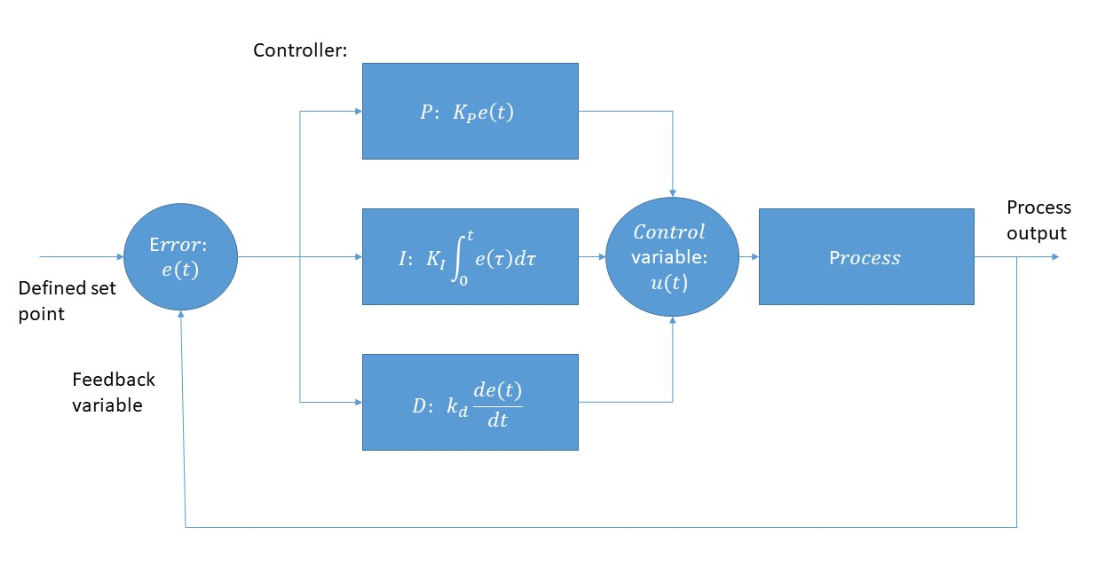
\includegraphics[scale=0.4]{\main/images/2 - theoretical background/pid_diagram_powerpoint.jpg}}
	\caption[PID controller block diagram]{PID controller block diagram}
	\label{fig:PID_scheme}
\end{figure}
\FloatBarrier
Proportional–integral–derivative (PID) controller is a feedback based control system. The control loop is used for time continuous control of a process, so the process output is close to a defined set point.
\par\noindent
PID controller continuously calculates error value, which is the difference of the process output from the defined set point. The feedback applies an external correction to the process, called control variable. The control variable is based on a gain to the error of proportional $P$, integral $I$ and derivative $D$. Proper tuning of a PID enables an accurate automated correction to a controlled process. The PID concept is used widely in applications requiring accurate automated control.

\par\noindent
The error and its integral and derivate are calculated continuously. The control has three tuning parameters; $K_P, K_I, K_D$, the feed back correction is modulated by the tuning parameters' value. Each parameter is assigned to a gain (P-I-D). The response (control variable) is a weighted sum of the control terms. Over time the controller attempts to minimize the error $e(t)$ by adjusting the control variable $u(t)$, which is the PID output.
\par\noindent

\begin{equation}
u(t) = K_P e(t)+K_I\int_{0}^{t}e(\tau)d\tau+K_D\frac{de(t)}{dt}   \label{eqn:PID_eqn}
\end{equation}

\noindent
$P$ is proportional to the current error value $e(t)$. When error is large and positive, proportional output would be proportionately large and positive.
\par\noindent
$I$ is proportional to past error value's integration. The response of the cumulative value could eliminate residual errors, such as signal offset.
\par\noindent
$D$ is proportional to error current change rate, by calculating the derivative. The response of the change rate could eliminate more rapid changes.
\par\noindent
The optimal control function is achieved by balancing the responses. The tuning constants depend on the characteristics of the specific process. The response must be tuned for each control application.  


\end{document}







